\documentclass{llncs}

% \usepackage[a4paper, left=2.5cm, right=2.5cm]{geometry}
\usepackage{listings}
\usepackage{amsmath}
\usepackage{amsfonts}
\usepackage{amssymb}
\usepackage{mathrsfs}

% use float package to provide supprot for position option H (in figure env)
\usepackage{float}
\usepackage{afterpage}

\usepackage{tikz}
\usepackage{pgf}
\usepackage{reotex}
\usepackage{subfigure}
\tikzset{
    state/.style={
           rectangle,
           rounded corners,
           draw=black, very thick,
           minimum height=2em,
           inner sep=2pt,
           text centered,
           },
}

\newcommand{\sem}[1]{$[\![{#1}]\!]$}
% todo: what is the proper name of the new model ?
\newcommand{\nSTA}{\mbox{STA}_r}

\begin{document}

\begin{example}[Embedded system]
The embedded system comprises a processor, sensors and an actuator.
The main processor, connected to ports \emph{$M_{in}$} and \emph{$M_{out}$},
reads data coming from sensors, and passes instructions to the actuator
through port \emph{Input} and \emph{Output}, respectively.
The system fails to get an input only when no data flows
    through each probabilistic filter.
A complete round, which starts when a data comes in
and stops when the output data is written successfully,
should be accomplished in a certain period of time,
otherwise the system sends out a timeout signal.

\begin{figure}[H]
    \centering
    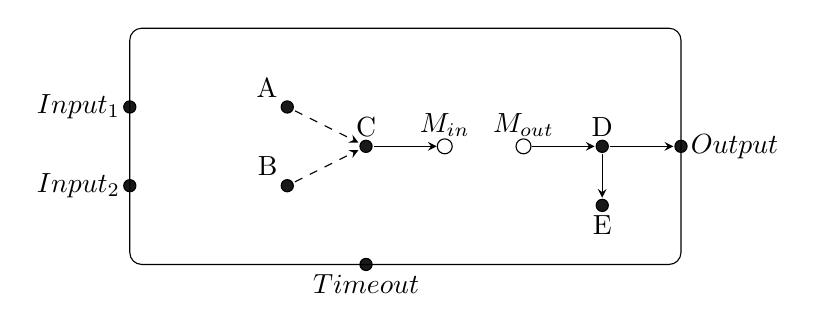
\begin{tikzpicture}
    \mixednode{(i1)}{(1, 1)}{node[left] {$Input_1$}}
    \mixednode{(i2)}{(1, 0)}{node[left] {$Input_2$}}

    \mixednode{(a)}{(3, 1)}{node[above left] {A}}
    \mixednode{(b)}{(3, 0)}{node[above left] {B}}

    \mixednode{(c)}{(4, 0.5)}{node[above ] {C}}
    \mixednode{(f)}{(4, -1.)}{node[below] {$Timeout$}}

    \mixednode{(d)}{(7, 00.5)}{node[above] {D}}
    \mixednode{(e)}{(7, -.25)}{node[below] {E}}

    \mixednode{(o)}{(8, 0.5)}{node[right] {$Output$}}

    \ionode{(m1)}{(5, 0.5)}{node[above] {$M_{in}$}}
    \ionode{(m2)}{(6, 0.5)}{node[above] {$M_{out}$}}

    \blackbox{(i1)}{(a)}{PF}{}
    \blackbox{(i2)}{(b)}{PF}{}

    \lossysync{(a)}{(c)}{}
    \lossysync{(b)}{(c)}{}

    \sync{(c)}{(m1)}{}
    \sync{(m2)}{(d)}{}

    \vrtimer{(c)}{(e)}{(f)}{RT}{}

    \sync{(d)}{(e)}{}
    \sync{(d)}{(o)}{}

    \component{(1,-1)}{(8,2)}{}

\end{tikzpicture}

    \caption{Embedded System}
    \label{fig:em}
\end{figure}

A \emph{probabilistic filter}, \textbf{PF} in short,
    drops data with a certain probability, i.e. $1 - p$; while
\textbf{RT} with time bound $t_{max}$,
which stands for \emph{reset timer}, can be reset.

\begin{figure}[H]
    \centering
    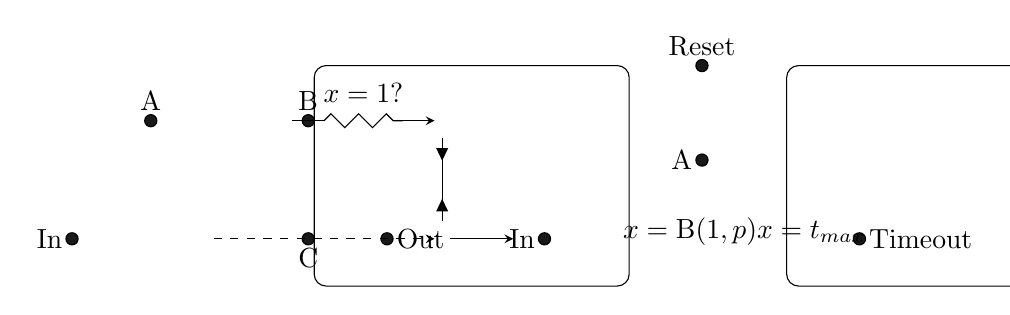
\begin{tikzpicture}
    %probabilistic filter
    \mixednode{(in1)}{(-7, 0)}{node[left] {In}}
    \mixednode{(a1)}{(-6, 1.5)}{node[above] {A}}
    \mixednode{(b1)}{(-4, 1.5)}{node[above] {B}}
    \mixednode{(c1)}{(-4, 0)}{node[below] {C}}
    \mixednode{(out1)}{(-3, 0)}{node[right] {Out}}

    %reset timer
    \mixednode{(in2)}{(-1, 0)}{node[left] {In}}
    \mixednode{(a2)}{(1, 1)}{node[left] {A}}
    \mixednode{(r2)}{(1, 2.2)}{node[above] {Reset}}
    \mixednode{(out2)}{(3, 0)}{node[right] {Timeout}}

    \choice{(in1)}{(a1)}{node [below right] {$x=\mathrm B(1, p)$}}
    \lossysync{(in1)}{(c1)}{}
    \sync{(c1)}{(out1)}{}
    \syncdrain{(b1)}{(c1)}{}
    \filter{(a1)}{(b1)}{node [above=3] {$x=1?$}}

    \choice{(r2)}{(a2)}{node [above right, xshift=0.1cm] {$x=t_{max}$}}
    \ptimer{(in2)}{(a2)}{(out2)}{}

    \component{(-7, -0.6)}{(-3, 2.2)}{}
    \component{(-1, -0.6)}{(3, 2.2)}{}

\end{tikzpicture}

    \caption{Probablistic Filter (left) and Reset Timer (right)}
    \label{fig:em}
\end{figure}

There are 8 locations in the $\nSTA$ of the embedded system,
consisting of triples which symbolizes the configuration of
    two probabilistic filters and the reset timer.
The $\nSTA$ is represented by \emph{JANI};
elements are ommited except locations and edges.

\lstinputlisting[language=Java]{em.jani}

\end{example}
\end{document}
